\newcommand{\sqrtFig}[1]{
    \pgfmathsetmacro{\off}{#1}
    \pgfmathsetmacro{\xmax}{1}
    \draw (-\xmax,0) -- (\xmax,0);
    \draw[domain=-\xmax:\xmax, smooth, variable=\x]  plot ({\x},{\x*\x+#1});
}%
\newcommand{\drawRoots}[1]{
    \pgfmathsetmacro{\ra}{-sqrt(#1)}
    \pgfmathsetmacro{\rb}{sqrt(#1)}
    \tkzDefPoints{\ra/0/R1, \rb/0/R2}
    \tkzDrawPoints(R1,R2)
}%
\tabulinesep=1mm%
\begin{tabu} to .9\linewidth {X[c]X[c]X[c]}
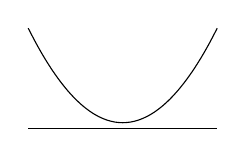
\begin{tikzpicture}[scale=1.2]
\sqrtFig{0.06}
\end{tikzpicture} &
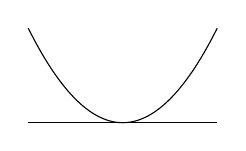
\begin{tikzpicture}[scale=1.2]
\sqrtFig{0}
\drawRoots{0}
\end{tikzpicture} &
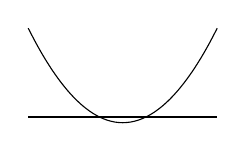
\begin{tikzpicture}[scale=1.2]
\sqrtFig{-0.06}
\drawRoots{0.06}
\end{tikzpicture}\\
$x^2-2x+(1+\epsilon) = 0$ & $x^2-2x+1 = 0$ & $x^2-2x+(1-\epsilon) = 0$\\
%$\Delta < 0$ & $\Delta = 0$ & $\Delta > 0$\\
no solution & $x = 1$ & $x = 1 \pm \sqrt{\epsilon}$\\
\end{tabu}
